\documentclass{beamer}
%\usetheme{Madrid}
\usepackage[utf8]{inputenc}
\usepackage{alltt}
\usepackage{graphicx}
\usepackage{hyperref}
\usepackage{listings}
\beamertemplatenavigationsymbolsempty
\setbeamertemplate{enumerate items}[ball]
\setbeamertemplate{frametitle}{\vspace*{0.5em}\hfill\insertframetitle}

\newcommand{\rd}[1]{\textcolor{red}{#1}}
\newcommand{\bl}[1]{\textcolor{blue}{#1}}
\newcommand{\mt}[1]{\ensuremath{\mathtt{#1}}}
%\newcommand{\rouge}[1]{{\color{orange}#1}}
\newcommand{\bleu}[1]{{\color{blue}#1}}
\newcommand{\monvert}[1]{{\color{blue}#1}}
\newcommand{\ocamlgraph}{\textsf{OCamlGraph}}
\newcommand{\vara}{\ensuremath{\alpha}}
\newcommand{\varb}{\ensuremath{\beta}}
\newcommand{\excode}[1]{\monvert{\texttt{#1}}}
\newcommand{\present}{{\monvert{\large\boldmath $\surd$}}}
\newcommand{\absent}{\textcolor{red}{\large\boldmath $\oslash$}}
\let\emph\alert

\lstdefinelanguage{ocaml}
{
basicstyle=\ttfamily,
morekeywords=[1]{module,struct,end,val,sig,let,type,functor,with,include},%
keywordstyle=[1]{\color{blue!80}},%
commentstyle=\itshape,%
columns=[l]fullflexible,%
sensitive=true,%
morecomment=[s]{(*}{*)},%
escapeinside={*?}{?*},%
keepspaces=true,
literate=%
%{'a}{$\alpha$}{1}%
%{'b}{$\beta$}{1}%
{<}{$<$}{1}%
{>}{$>$}{1}%
{<=}{$\le$}{1}%
{>=}{$\ge$}{1}%
{<>}{$\ne$}{1}%
{/\\}{$\land$}{1}%
{\\/}{ $\lor$ }{3}%
{\ or(}{ $\lor$(}{3}%
% {not\ }{$\lnot$ }{1}%
% {not(}{$\lnot$(}{1}%
{+->}{\texttt{+->}}{2}%
% {+->}{$\mapsto$}{2}%
{-->}{\texttt{-\relax->}}{2}%
%{-->}{$\longrightarrow$}{2}%
{->}{$\rightarrow$}{2}%
{<-}{$\leftarrow$}{2}%
{<->}{$\leftrightarrow$}{2}%
%
%
}
\lstnewenvironment{ocaml}{\lstset{language=ocaml}}{}
\newcommand{\of}[1]{\lstinline[language=ocaml]{#1}}

\title{Lessons from the implementation of a graph library, OCamlGraph}
\author{Jean-Christophe Filli\^atre}
\institute{CNRS}
\date{Meetup OCaml-Paris (OUPS) \\ July 8, 2014}

\begin{document}
\addtocounter{framenumber}{-1}

\maketitle

\setbeamertemplate{footline}{\vspace*{-0.5em}\hfill \color{blue}OCamlGraph --- \insertframenumber/\inserttotalframenumber}

\begin{frame}\frametitle{OCamlGraph}

  \begin{description}
  \item[what] a graph library for OCaml \\
    LGPL 2.1 + special exception for linking

    \bigskip
    \item[when]
      started in 2004

    \bigskip
  \item[who] Sylvain Conchon (Univ Paris Sud) \\
    Jean-Christophe Filliâtre (CNRS) \\
    Julien Signoles (CEA) \\
    + external contributors

    \bigskip
    \item[where]
    \url{http://ocamlgraph.lri.fr/} \\
    code on github
  \end{description}
\end{frame}

\begin{frame}\frametitle{overview}
  \begin{itemize}
  \item using OCamlGraph
    \begin{itemize}
    \item data structures
    \item algorithms
    \end{itemize}
    \vskip15pt
  \item implementing OCamlGraph
    \vskip15pt
  \item lessons
  \end{itemize}
\end{frame}

%%%%%%%%%%%%%%%%%%%%%%%%%%%%%%%%%%%%%%%%%%%%%%%%%%%%%%%%%%%%%%%%%%%%%%%%%%%%%%%

%\section[Interface]{}

\begin{frame}[containsverbatim]
  \frametitle{what kind of graphs do you need?}

  \begin{itemize}
  \item mutable graph?
    \hfill \excode{Imperative} or \excode{Persistent}
    \vskip10pt
  \item directed?
    \hfill \excode{Digraph} or \excode{Graph}
    \vskip10pt
  \item labels on edges?
    \hfill \excode{Labeled} (or unlabeled)
    \vskip10pt
  \item abstract data type for vertices?
    \hfill \excode{Abstract} or \excode{Concrete}
    \vskip10pt
  \end{itemize}

\bigskip
\begin{center}
all 16 possibilities provided, as \emph{functors}
\end{center}
\end{frame}

\begin{frame}[fragile]
  \frametitle{examples}
  \begin{itemize}
  \item imperative directed graphs with integer vertices and unlabeled edges
\medskip
    \begin{ocaml}
module G =
  Imperative.Digraph.Abstract(struct type t = int end)
    \end{ocaml}

  \item persistent undirected graphs with string vertices and edges
\medskip
    \begin{ocaml}
module S = struct type t = string ... end
module G = Persistent.Graph.ConcreteLabeled(S)(S)
    \end{ocaml}
  \end{itemize}
\end{frame}

% \begin{frame}[containsverbatim]
%   \frametitle{Interfaces}
%   \emph{Common interface for all graphs:}
%   \begin{alltt}
%     module type \bleu{G} = sig ... end
%   \end{alltt}
%   \emph{Interface for persistent graphs:}
%   \begin{alltt}
%     module type \bleu{P} = sig
%       include \bleu{G}
%       ...
%     end
%   \end{alltt}
%   \emph{Interface for imperative graphs:}
%   \begin{alltt}
%     module type \bleu{I} = sig
%       include \bleu{G}
%       ...
%     end
%   \end{alltt}
% \end{frame}


\begin{frame}\frametitle{19 graph data structures}
  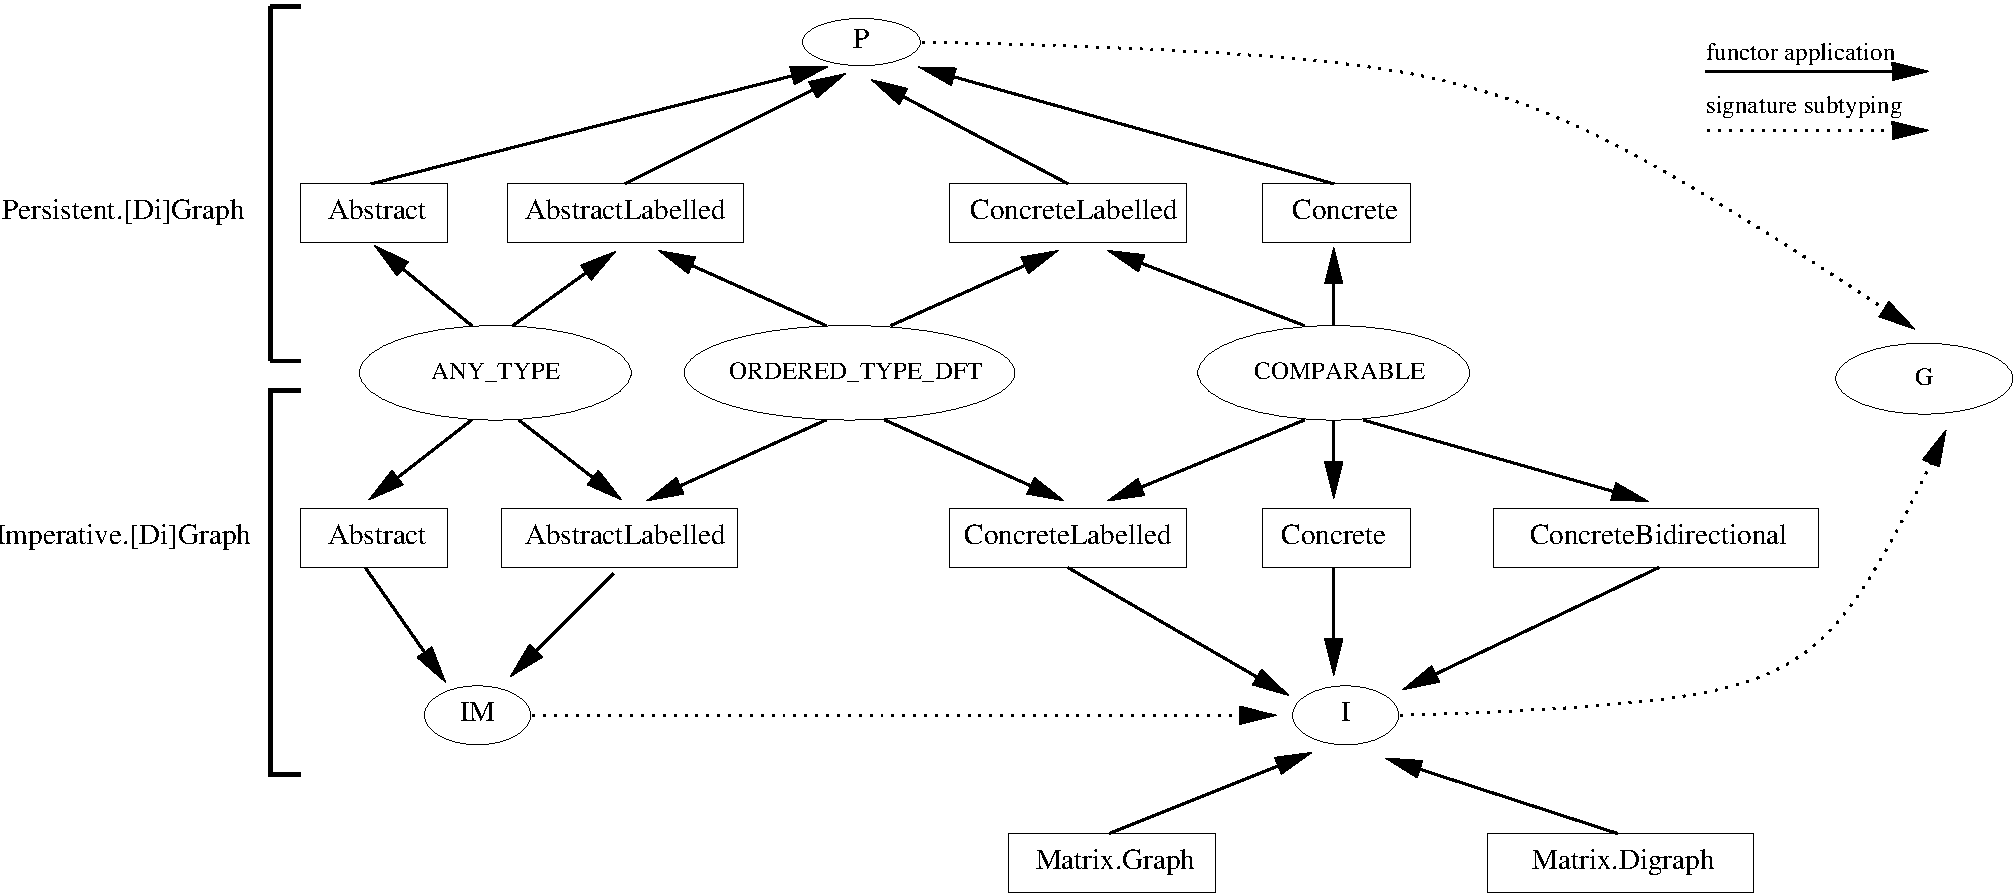
\includegraphics[width=\textwidth]{tfp07/interface.pdf}
%\vskip-1pt
\begin{itemize}
\item 8 \bleu{persistent}: implemented with AVLs
\item 8 \bleu{imperative}: implemented with hash tables
\item 3 \bleu{specialized}: adjacency matrices and bidirectional graphs
\end{itemize}
\end{frame}

\begin{frame}[fragile]
  \frametitle{graph operations}
  \begin{itemize}
  \item \emph{creation} (insertion, suppression, etc.)
    \begin{ocaml}
      val add_vertex : t -> vertex -> unit
    \end{ocaml}
  \item \emph{test functions}
    \begin{ocaml}
      val mem_edge : t -> vertex -> vertex -> bool
    \end{ocaml}
  \item \emph{iterators} (vertices, edges, successors, etc.)
    \begin{ocaml}
      val iter_vertex : (vertex -> unit) -> t -> unit
    \end{ocaml}
  \end{itemize}
\end{frame}

\begin{frame}
  \frametitle{graph algorithms}

  \begin{center}
    written independently of the graph implementation\\[1.2em]
    \emph{algorithm = functor}\\[1em]
  \end{center}
\end{frame}

\begin{frame}[fragile]
  \frametitle{example: shortest path}

  \begin{enumerate}
  \item \emph{instantiating} the functor
  \begin{ocaml}
    module W = struct
      type t = int
      let zero = 0
      let add = (+)
      ...
    end
    module Dij = Path.Dijkstra(G)(W)
  \end{ocaml}

  \item \emph{using} the resulting module
  \begin{ocaml}
    let path,w = Dij.shortest_path g v1 v2
  \end{ocaml}
  \end{enumerate}
\end{frame}

\begin{frame}[fragile]
  \frametitle{minimal functor signature}
only the \emph{required operations} as functor parameters
  \begin{ocaml}
module type G = sig
  type t
  module V : sig type t ... end
  module E : sig type t ... end
  val iter_succ_e : (E.t -> unit) -> t -> V.t -> unit
end
module Dijkstra
  (G: G)
  (W: sig type t val weight : G.E.t -> t ... end)
sig
  val shortest_path : G.t -> G.V.t -> G.V.t ->
                      G.E.t list * W.t
end
  \end{ocaml}
\end{frame}

\begin{frame}
  \frametitle{benefits of functorized algorithms}

  \begin{itemize}
  \item clearly \emph{separates} algorithms from data structures\vskip8pt
  \item possible use on \emph{non-\ocamlgraph} data structures\vskip8pt
  \item easy \emph{extension} with new algorithms\vskip8pt
  \end{itemize}

\end{frame}

\begin{frame}
  \frametitle{some algorithms in \ocamlgraph}
  \begin{itemize}
  \item traversal: 7 DFS, 2 BFS, 2 cycle detections
  \item topological sorting
  \item strongly connected components
  \item shortest path: Dijkstra, Bellman-Ford
  \item minimum spanning tree: Kruskal, Prim
  \item maximal flow: Goldberg, Ford-Fulkerson
  \item $k$-coloring
  \item transitive closure, complement, mirror,
    neighborhood, \dots
  \item building:
    \begin{itemize}
    \item classic graphs (e.g. de Bruijn's)
    \item random graphs (e.g. planar graph)
    \end{itemize}
  \item interfaces with Graphviz and GML
\end{itemize}
\end{frame}

%%%%%%%%%%%%%%%%%%%%%%%%%%%%%%%%%%%%%%%%%%%%%%%%%%%%%%%%%%%%%%%%%%%%%%%%%%%%%%%

%\section[Implementation]{}

\begin{frame}
  \frametitle{overview}
  \begin{itemize}
  \item \textcolor{black!30}{using OCamlGraph\vskip15pt}
  \item implementing OCamlGraph\vskip15pt
  \item \textcolor{black!30}{lessons\vskip15pt}
  \end{itemize}
\end{frame}

\begin{frame}
  \frametitle{software engineering}
  \begin{center}
    how to code and to maintain 19 graph implementations?
  \end{center}
\end{frame}

\begin{frame}
  \frametitle{factorizing code with functors}
  \begin{itemize}
  \item
    abstracting the underlying implementation (AVL or hash table) by using a
    common signature \excode{HM}

  \vskip8pt
  \item
    one functor for each feature
    \vskip1pt
    \begin{itemize}
    \item \excode{Minimal}: common operations
      \vskip6pt
    \item \excode{Labeled}/\excode{Unlabeled}
      \vskip6pt
    \item \excode{Pred}: predecessors from successors
      \vskip6pt
    \item \excode{Make\_Abstract}: abstract graphs from concrete ones
    \end{itemize}
  \end{itemize}
\end{frame}

\begin{frame}[containsverbatim]
  \frametitle{example}

persistent or imperative unlabeled directed graphs

\begin{ocaml}
module Make
  (F: functor(X: COMPARABLE) -> HM with type key = X.t) =
struct
  module Digraph = struct
    module Concrete(V: COMPARABLE) = struct
      include ConcreteVertex(F)(V)
      include Unlabeled(V)(HM)
      include Minimal(S)(HM)
    end
end
module I = Make(Make_Hashtbl)
module P = Make(Make_Map)
\end{ocaml}
\end{frame}

\begin{frame}
  \frametitle{code factorization}

  altogether,

  19 data structures $\times$ 45 operations each = 855 operations

  \bigskip
  only \emph{1,000 lines} of code
\end{frame}


%%%%%%%%%%%%%%%%%%%%%%%%%%%%%%%%%%%%%%%%%%%%%%%%%%%%%%%%%%%%%%%%%%%%%%%%%%%%%%%


\begin{frame}
  \frametitle{overview}
  \begin{itemize}
    \item \textcolor{black!30}{using OCamlGraph\vskip15pt
    \item implementing OCamlGraph\vskip15pt}
  \item lessons
  \end{itemize}
\end{frame}

% \begin{frame}
%   \frametitle{comparison}
%   \begin{center}
%   \begin{tabular}{|l||c|c|c|c|c|}
%     \hline
%      Library & Language     &P/I& Genericity & Data struct. \\\hline\hline
%      GTL & C++     & I & \absent  & 1  \\\hline
%      LEDA & C++    & I & \absent  & 2  \\\hline
%      BGL & C++     & I & \present & 2  \\\hline
%      JDSL & Java   & I & \present & 1  \\\hline
%      FGL & Haskell & P & \absent  & 1  \\\hline
%      MLRisc & SML  & I & \absent  & 1  \\\hline
% %     Baire & Ocaml &P/I& ---      & 8  \\\hline
%      \emph{\ocamlgraph}& Ocaml &P/I& \present & \emph{19} \\\hline
%   \end{tabular}
%   \end{center}
% \end{frame}

\begin{frame}\frametitle{lesson 1: make it simple}
  \begin{itemize}
  \item simple
    \begin{itemize}
    \item initially 9 men-weeks
    \item 7,000 loc (later 2,000 loc by external contributors)
    \end{itemize}
    % \begin{center}
    %   \emph{only possible thanks to ML functors}
    % \end{center}\vskip10pt

    \bigskip
  \item yet efficient
    \begin{itemize}
    \item creation $\approx$ 100,000 edges per second
    \item traversal $\approx$ 1 million edges per second
    \end{itemize}
    % \begin{center}
    %   \emph{compares well to other graph libraries}
    % \end{center}
  \end{itemize}
\end{frame}

\begin{frame}\frametitle{lesson 1: make it simple}
  \begin{itemize}
  \item \emph{the first principle of optimization is \textit{don't}} \par
    (Kernighan \& Pike, \textit{The Practice of Programming})

  \bigskip
  \item implement algorithms as in textbooks
    \begin{itemize}
    \item iterators and functors make it easy
    \end{itemize}

  \bigskip
  \item yet, don't be naive when it comes to data structures
    \begin{itemize}
    \item do care about complexity
    \end{itemize}
  \end{itemize}
\end{frame}

\begin{frame}\frametitle{lesson 2: functors}
  there are modules and functors all over the place

  (450 occurrences of the \of{module} keyword)

  \bigskip
  \begin{itemize}
  \item a few bugs/limitations of the module system
    \begin{itemize}
    \item cf BTS \#2049 (weakness of applicative modules)
    \item two signatures with a common type or a module
    \end{itemize}
  \end{itemize}
\end{frame}

\begin{frame}\frametitle{lesson 2: functors}
  too many functors in the API can be a pain for the user

  \bigskip
  \begin{itemize}
    \item many functors are used internally only

      \bigskip
    \item a module \of{Pack} provides a simple API, with no functor
      \begin{itemize}
      \item one particular graph data structure
      \item all functors already applied for you
      \end{itemize}

  \bigskip
  \item refrain yourself from making everything as generic as possible
  \end{itemize}
\end{frame}

\begin{frame}
  \begin{center}
    questions ?
  \end{center}
\end{frame}

\end{document}


% Local Variables:
% compile-command: "rubber -d oups-july-2014"
% ispell-local-dictionary: "american"
% End:
